\graphicspath{ {Context/Images/} }


\chapter{Context}
\label{cha:context}

\section{Introduction}
In this chapter 

Context: Depends on chosen problem (Extracting knowledge from EHR )

	Problem: info out of EHR
	State of the art:
	
		Explain Disease codes
		DiseaseProgression
		Explain Danish paper, Matrix group America (recommender), Querying


\section{Electronic Health Records}

An electronic health record (EHR) is a collection of time-stamped data about a patient over a period point of time. It is stored digitally and thus can be established for a large number of patients over a long time period. \\
The data stored in an EHR provides an overview of the patients health information. Health information like demographics, medical history, diagnoses, medications, and such, are stored \cite{HealthIT:online}. \\

Large countries like the US and the UK, are each investing more than $20$ billion dollars into EHR systems \cite{EHRworld:article}. Those systems are adopted by around $70$\% of the physicians. Which means a large number of physicians are using other methods or systems. Also, each country develops his own system which results in a good nationwide coverage but introduces different system around the world. We focus on disease codes in the next section and introduce two standards: one used by mainly insurance companies and the other used by pharmaceutical companies.


\subsection{Disease Codes}

To make EHRs practical it is important to adhere to standards for data formatting. A well documented standard makes it easy to store and extract information from large-scale databases of EHRs. Without the possibility of extracting information, an EHR becomes a simple digital version of medical records on paper. \\
A part of an EHR consists of the diagnosis of the patient. It provides information about his disease trajectory and allows analysis on his health situation. With a uniform system for classifying diseases, it is possible to provide a general picture on health situations of populations.

\subsubsection{ICD-10}

The International Statistical Classification of Diseases and Related Health Problems (ICD) is a medical classification list made by the World Health Organization (WHO) \cite{WHO_ICD:online}. The ICD-10 contains more than $14,400$ codes about diseases, disorders, injuries, and other related health conditions. For example, the code for a sprained ankle is $S93.4$. It also provides hierarchical categories for those codes to allow a more general overview of diseases. ICD is mainly used by insurance companies.


\subsubsection{MedDRA}

The Medical Dictionary for Regulatory Activities (MedDRA) provides medical terminology in the form of disease codes \cite{MedDRA:online}. A MedDRA code is an eight digit numberic code where new terms are assigned sequentially. It does not provide clear hierarchical categories like ICD which can't be understand without a medical background. MedDRA is mainly used by pharmaceutical companies.

\section{EHR Analytics}

EHRs provide a massive amount of data which could be used to create useful insights. The data contains the medical history of a patient including medical measurements, diagnosis, prescribed drugs, and demographics. Based on those values, we could obtain the following insights:

\begin{itemize}

\item Effects of drugs
\item Medical costs for certain diseases
\item Duration and recovery percentage of certain diseases
\item Correlation between demographics and certain diseases
\item Link between current health state and health history
\item Prediction of future health states based on history

\end{itemize}

Those insights can be offered on an individual level, which means a right intervention to the right patient at the right time. EHR analytics can be used to have a personalized care and benefits the healthcare system by cutting costs and improve outcomes. \\

In the following sections we talk about current EHR analytic methods.


\subsection{Querying}

Analytics in epidemiology on EHRs is typically done through querying a database \cite{EHRquery:journal}. A specialist can have a certain idea about correlations between conditions or patients. He can support this idea by finding cases in EHRs and analyzing the results of his query. \\
This method is based on the knowledge and experience of a specialist. The information has to be actively sought after and unexpected or complex correlations are not considered. Some complex relations cannot be found because of the limitations of the querying language. A query language is equivalent to first-order logic. Which means non-linear relations in the data cannot be found.

\subsection{Big Data Analytics}

More advanced methods are applied on EHR than querying. In general, they try to find patterns in the EHR data which then can be used to predict outcomes of treatments \cite{EHRbigdata:slides}. \\

Several predictive methods can be used and show promising results \cite{EHRmining:article}. Those results are achieved by using non-optimized methods which are applied on the EHR data. We also note that methods used as Multi-layer Perceptron networks are not ideal for prediction of time-series, see section \ref{sec:PatientClassification}. We conclude that there is still a lot of room for improvement. \\
 
More specialized approaches are also applied on EHR data \cite{EHRrecommender:article}. 
An EHR of a patient can be transformed into a matrix structure, see figure \ref{fig:matrixPatient}. On these matrix structures, feature extraction methods can be applied similar to recommender systems. This can, for example, be done by defining patient similarities \cite{EHRsimilarity:article}. So when a patient is similar to a previous patient, his treatment can be based on previous experiences.

\begin{figure}[H]
	\centering
	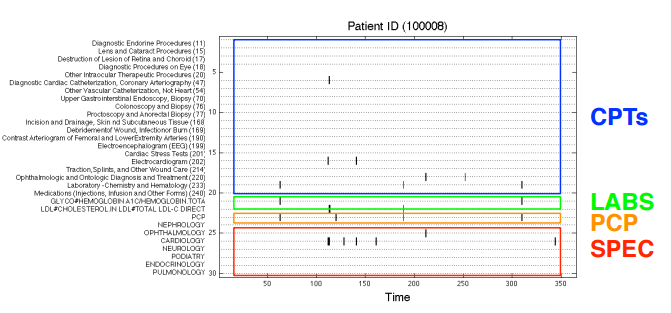
\includegraphics[width=\textwidth]{matrixPatient.png}
	\caption{Example of an EHR transformed into a matrix structure \cite{EHRrecommender:article}}
	\label{fig:matrixPatient}
\end{figure}


\subsection{Statistical Analysis}

A combination of statistical methods and graph clustering are applied to obtain disease trajectories. To have any significance using those methods, a large set of EHRs need to be used. \\
These techniques have been applied to Danish EHRs. The study identifies temporal correlations between pairs of diagnoses. The pairs are further clustered into larger disease trajectories based on the diagnoses they shared. Based on the clusters, patients can be categorized into certain trajectories and retrieve a more personal care. An example of a cluster graph can be found in figure \ref{fig:clusterGraphDanish}.

\begin{figure}[H]
	\centering
	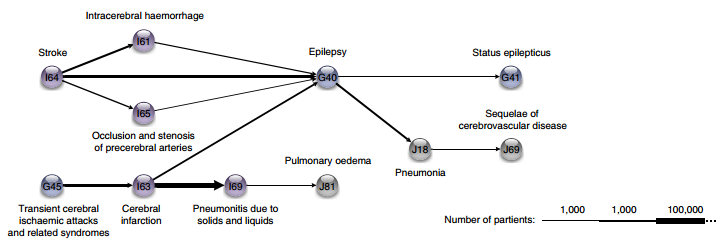
\includegraphics[width=\textwidth]{clusterGraphDanish.png}
	\caption{Cerebrovascular disease trajectory cluster for the Danish population \cite{Brunak:article}}
	\label{fig:clusterGraphDanish}
\end{figure}

http://www.nature.com/ncomms/2014/140617/ncomms5022/pdf/ncomms5022.pdf


\section{Conclusion}
The final section of the chapter gives an overview of the important results
of this chapter. This implies that the introductory chapter and the
concluding chapter don't need a conclusion.



%%% Local Variables: 
%%% mode: latex
%%% TeX-master: "thesis"
%%% End: 
